\documentclass[border=10pt]{standalone}
\usepackage{tikz}\usepackage{amsmath}
\usetikzlibrary{calc,arrows.meta}
\begin{document}
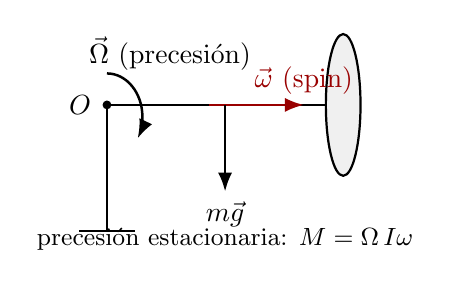
\begin{tikzpicture}[line width=0.9pt,>={Latex[length=2.4mm]}]
  % soporte vertical
  \draw[thick] (0,-1.6)--(0,0);
  \draw[thick] (-0.35,-1.6)--(0.35,-1.6);
  \fill (0,0) circle(1.6pt) node[left=2pt]{$O$};
  % eje del rotor (horizontal)
  \draw[thick] (0,0)--(3.0,0);
  % disco (rotor) al final
  \draw[thick,fill=black!6] (3.0,0) ellipse (0.22 and 0.9);
  % spin
  \draw[->,red!60!black] (1.3,0)--(2.5,0) node[above]{$\vec\omega$ (spin)};
  % peso
  \draw[->] (1.5,0)--(1.5,-1.1) node[below]{$m\vec g$};
  % precesion (vertical)
  \draw[->] (0,0.4) arc (90:-30:0.45 and 0.55); \node at (0.8,0.65){$\vec\Omega$ (precesión)};
  \node at (1.5,-1.7){\small precesión estacionaria: $M=\Omega\,I\omega$};
\end{tikzpicture}
\end{document}
